\subsubsection{Decomposi\c c\~ao STL}

\citeonline{Theodosiou20111178} A decomposição sazonal e tendencial utilizando o procedimento de Loess (STL) é utilizada para a decomposição aditiva da série temporal global. O STL realiza a decomposição aditiva dos dados por meio de uma sequência de aplicações do Loess mais suave, que aplica regressões polinomiais ponderadas localmente em cada ponto do conjunto de dados, sendo as variáveis explicativas os valores mais próximos do ponto cuja resposta está sendo estimada. 

\begin{figure}[H]
	\centering
	\caption{Decomposição STL aditiva dos dados coletados}
	\label{fig:stl-aditiva}
	\includegraphics[width=0.9\linewidth]{"Resultados/Figuras/STL aditiva"}
	
	Fonte: Elaboração própria a partir de dados da SANEPAR (2018 a 2020)
\end{figure}


\begin{figure}[H]
	\centering
	\caption{Decomposição STL multiplicativa dos dados coletados}
	\label{fig:stl}
	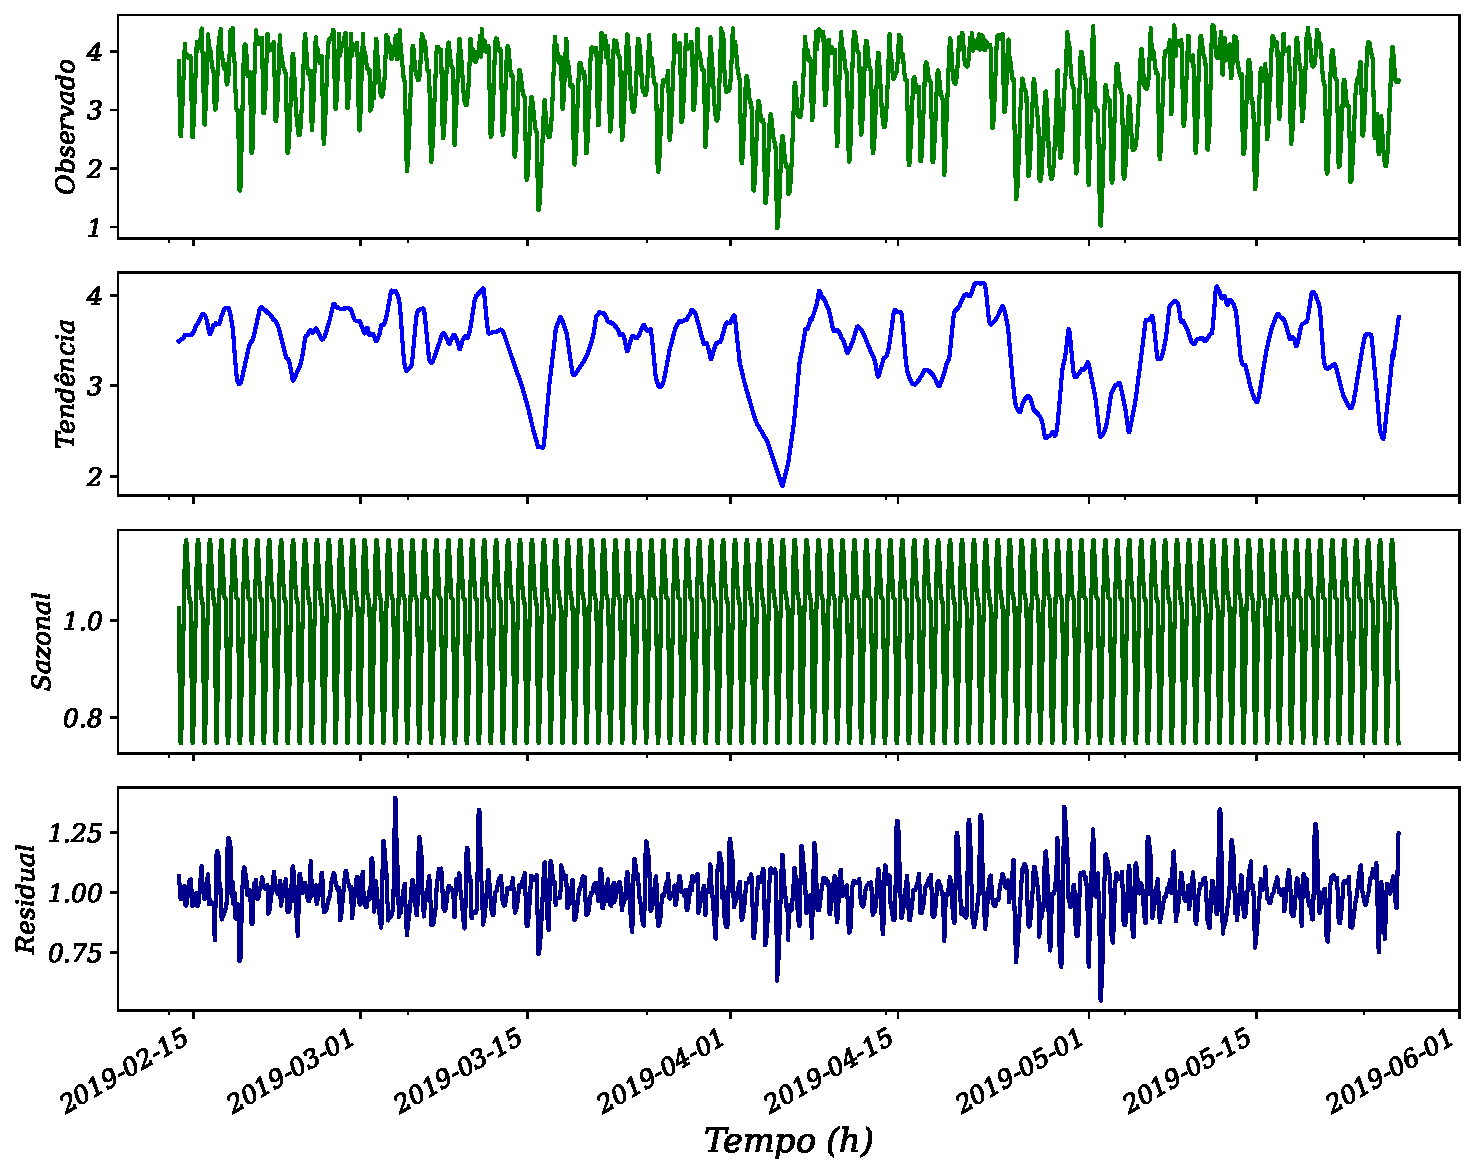
\includegraphics[width=0.9\linewidth]{Resultados/Figuras/STL}
	
	Fonte: Elaboração própria a partir de dados da SANEPAR (2018 a 2020)
\end{figure}

Na \ref{q5}\ref{q5:b} resposta pode ser dada pelas Figuras \ref{fig:stl-aditiva} e \ref{fig:stl} como é observado tem tenacidade, sazonalidade e resido. 

Na decomposição, o objetivo é analisar se há tenacidade, sazonalidade e residência, olhando as Figuras \ref{fig:stl-aditiva} e \ref{fig:stl}, mostra que os dados têm ambas as análises. E com isso percebe-se que a série é estacionária, através do seguinte teste.

Teste de Dickey-Fuller (DF) Aumentado: 
\begin{itemize}
	\item Estatística de teste ADF     $-4.248$
	\item $p-valor$                       $0.001$
	\item atrasos utilizados         $21.000$
	\item  observações              $1074.000$
	\item valor crítico $(1\%)           -3.436$
	\item valor crítico $(5\%)           -2.864$
	\item valor crítico $(10\%)          -2.568$
	
	
	Forte evidência contra a hipótese nula
	
	Rejeitar a hipótese nula
	
	Os dados não têm raiz unitária e estão estacionários em \ref{q5}\ref{q5:c}, pois a série está estacionária para identificar quais são as horas de pico entre 18h e 21h não é um trabalho fácil, como se você levasse a Figura \ref{fig:hist} para ver que no ano de 2020 houve um aumento na demanda naquelas horas.
	
	
	\begin{figure}[H]
		\centering
		\caption{Violino no nível do reservatório}
		\label{fig:hist}
		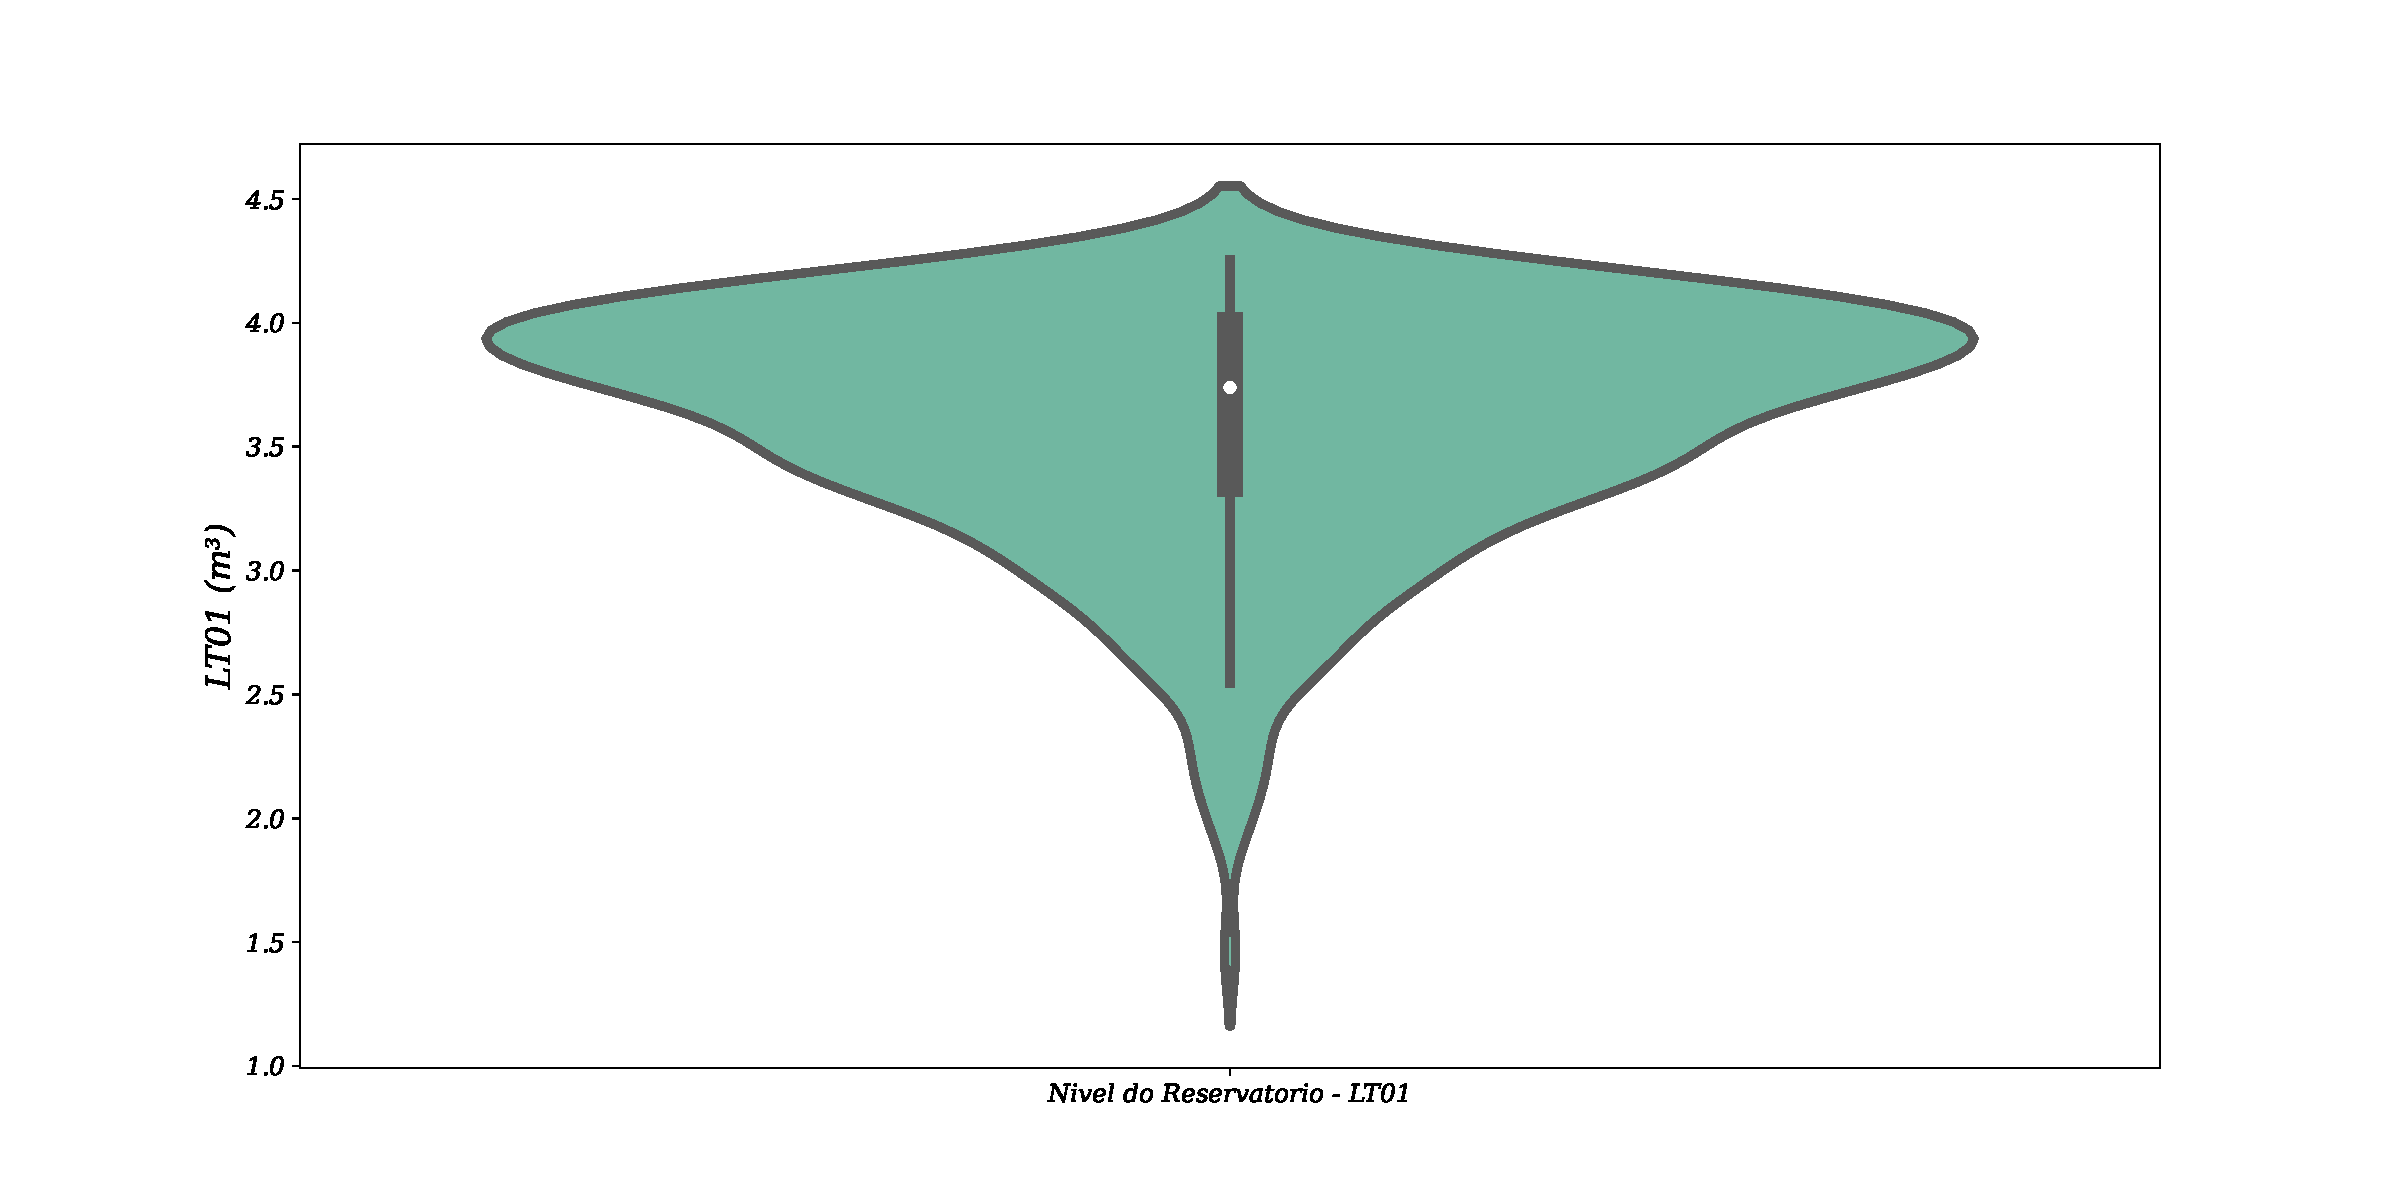
\includegraphics[width=0.9\linewidth]{Resultados/Figuras/viol}
		
		Fonte: Elaboração própria a partir de dados da SANEPAR (2018 a 2020)
	\end{figure}
	
	Assim, como dito na seção \ref{subsubsec:motivacao} as anomalias climáticas mais ocasionadas no ano 2020 e foi devido à falta de chuva naquele período.
	
	Em \ref{q5}\ref{q5:d} nas horas de pico deve conter no tanque cerca de $[3.545,4.256] m^3$ para que não ligue as bombas.
	
	
	\begin{figure}[H]
		\centering
		\caption{Violino da vazão de recalque}
		\label{fig:ft03}
		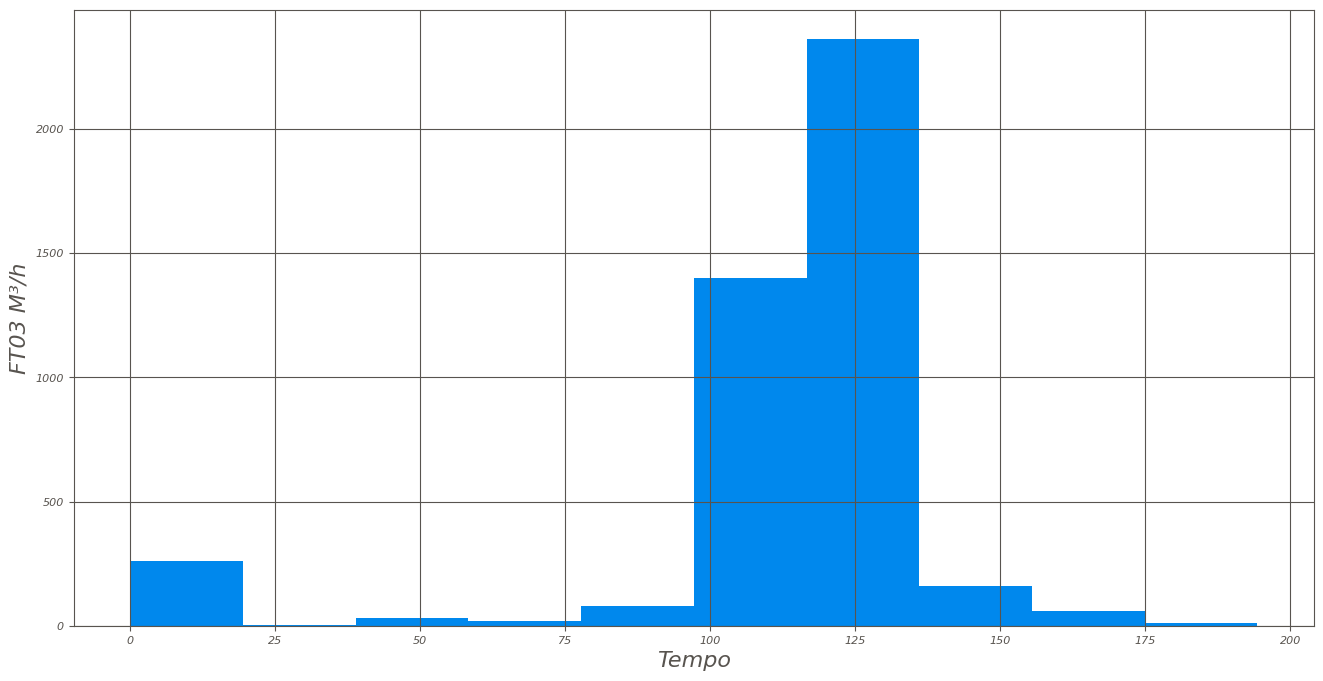
\includegraphics[width=0.9\linewidth]{Resultados/Figuras/ft03}
		
		Fonte: Elaboração própria a partir de dados da SANEPAR (2018 a 2020)
	\end{figure}
	
	Para \ref{q5}\ref{q5:e} é mostrado na Figura \ref{fig:ft03} como a vazão pode ser afetada com o nível do tanque. A vazão de recalque influencia mais o nível do tanque do que as outras vazões porque injeta água no tanque através da bomba que está mais próxima da base do tanque e as outras vazões por ter alguns valores ausentes não interferem tanto na amostra.
	
	
\end{itemize}

De acordo com o \citeonline{Reisen2017115}, o teste DF tem as seguintes equações

\begin{eqnarray}
	z_t&=& y_t+\theta \beta_t, \qquad t=1,\ldots, T, \label{eq:df3}\\	
	\hat{\rho}_{\mathrm{DF}}-1&=&\frac{\sum_{t=1}^T z_{t-1} \Delta z_t}{\sum_{t=1}^T z_{t-1}^2} \label{eq:regdf}
\end{eqnarray}

De \eqref{eq:regdf} onde $\Delta z_t=z_t-z_{t-1}$. Sob a hipótese nula $\left(H_0\right)$ : `` $\rho=1$'', as estatísticas do teste DF e suas distribuições limitantes são dadas da seguinte forma:


\begin{eqnarray}
	T\left(\hat{\rho}_{\mathrm{DF}}-1\right)=T \frac{\sum_{t=1}^T z_{t-1} \Delta z_t}{\sum_{t=1}^T z_{t-1}^2}
\end{eqnarray}
e


\begin{eqnarray}
	\hat{\tau}_{\mathrm{DF}}&=&\frac{\hat{\rho}_{\mathrm{DF}}-1}{\hat{\sigma}_{\mathrm{DF}}\left(\sum_{t=1}^T z_{t-1}^2\right)^{-1 / 2}} \label{eq:df}
\end{eqnarray}

De \eqref{eq:df} onde $\hat{\sigma}_{\mathrm{DF}}^2=T^{-1} \sum_{t=1}^T\left(\Delta z_t-\left(\hat{\rho}_{\mathrm{DF}}-1\right) z_{t-1}\right)^2 .$



Suponha que $\left(z_t\right)_{1 \leq t \leq T}$ são dadas por \eqref{eq:df3}, então quando $\rho=1$,


\begin{eqnarray}
	T\left(\hat{\rho}_{\mathrm{DF}}-1\right) \stackrel{d}{\longrightarrow} \frac{W(1)^2-1}{2 \int_0^1 W(r)^2 \mathrm{~d} r}-\left(\frac{\theta}{\sigma}\right)^2 \frac{\pi}{\int_0^1 W(r)^2 \mathrm{~d} r}, \text { como } T \rightarrow \infty \\
	\hat{\tau}_{\mathrm{DF}} \stackrel{d}{\longrightarrow}\left[1+2(\theta / \sigma)^2 \pi\right]^{-1 / 2}\left\{\frac{W(1)^2-1}{2\left(\int_0^1 W(r)^2 \mathrm{~d} r\right)^{1 / 2}}-\frac{(\theta / \sigma)^2 \pi}{\left(\int_0^1 W(r)^2 \mathrm{~d} r\right)^{1 / 2}}\right\} \\
	\quad \operatorname{como} T \rightarrow \infty\label{eq:df2}
\end{eqnarray}

A partir de \eqref{eq:df2}, onde$\stackrel{d}{\longrightarrow}$ denota convergência na distribuição e onde $\{W(r), r \in[0,1]\}$ denota o movimento Browniano padrão.

Este teste na literatura é chamado de teste ACF para testar se a série é estacionária ou não.

\begin{figure}[H]
	\centering
	\caption{Autocorrelação e Autocorrelação parcial}
	\label{fig:acf}
	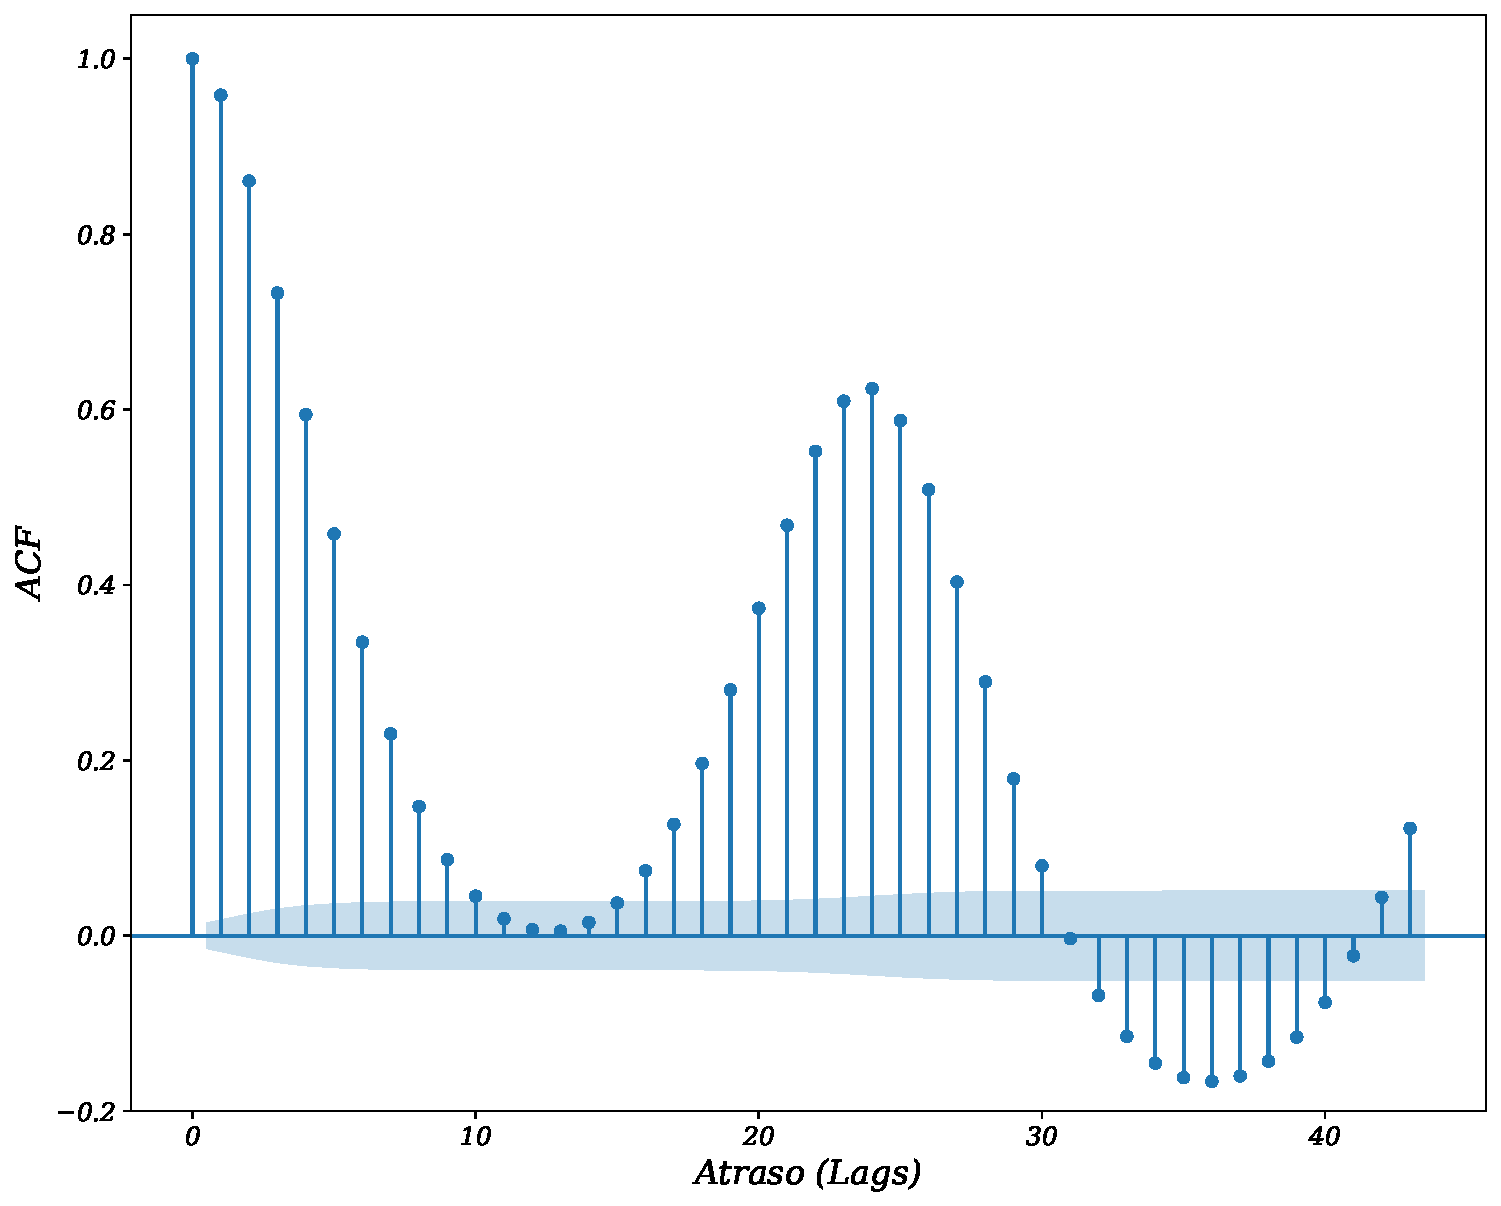
\includegraphics[width=0.9\linewidth]{Resultados/Figuras/acf} 
	
\end{figure}	
\begin{figure}[H]
	\centering
	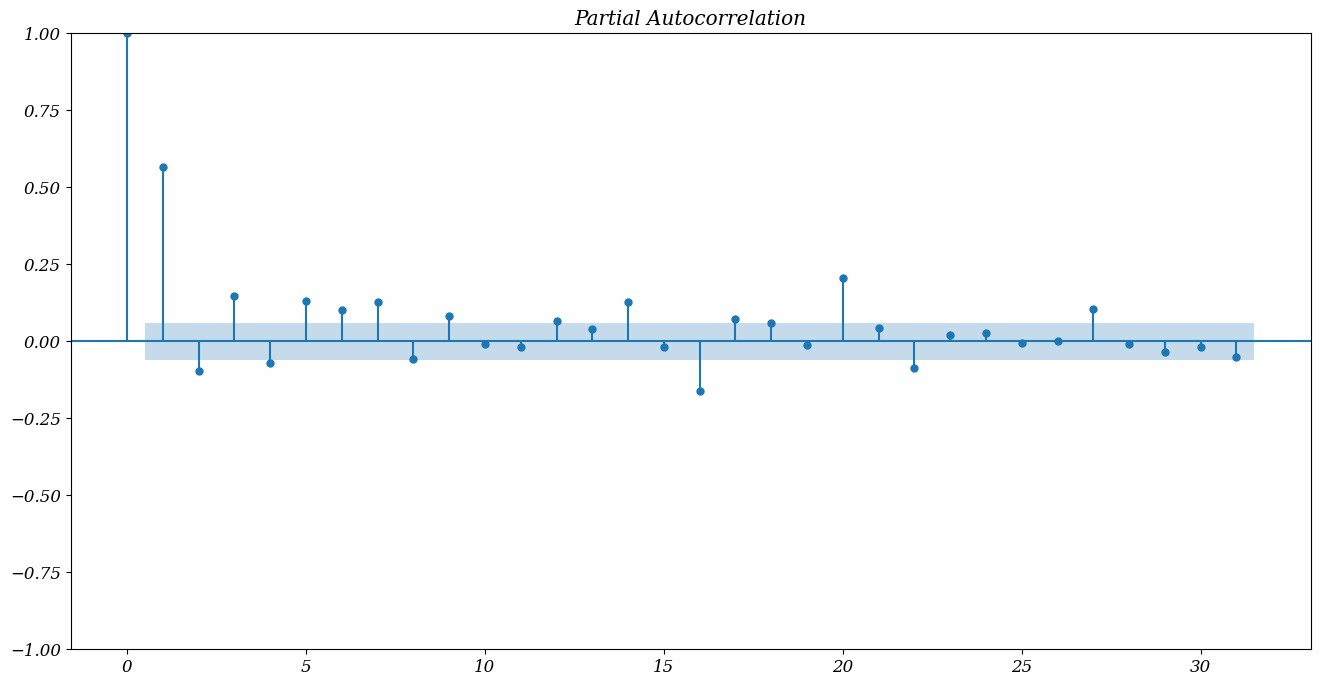
\includegraphics[width=0.9\linewidth]{Resultados/Figuras/pacf}
	
	Fonte: Elaboração própria a partir de dados da SANEPAR (2018 a 2020)
\end{figure}

Na figura \ref{fig:acf} temos a diferença entre autocorrelação e autocorrelação parcial (PACF) é quase um detalhe em um ACF temos a correlação direta e indireta e em um PACF somente a correlação direta.  

Na Figura \ref{fig:acf} tem a diferença entre a autocorrelação e a autocorrelação parcial (PACF) é quase um detalhe em uma ACF temos a correlação direta e indireta e em uma PACF apenas a correlação direta. 

O intervalo de confiança padrão é 95\% mostrado como esta marca azul. As observações que estão fora da marca são consideradas estatisticamente correlacionadas.

A correlação na Figura \ref{fig:acf} é a explicação do teste DF. Os valores de uma série de ruído branco são totalmente aleatórios, ou seja, este é um tipo de série que não é previsível.

\begin{figure}[H]
	\centering
	\caption{Ruído branco}
	\label{fig:ruido-branco}
	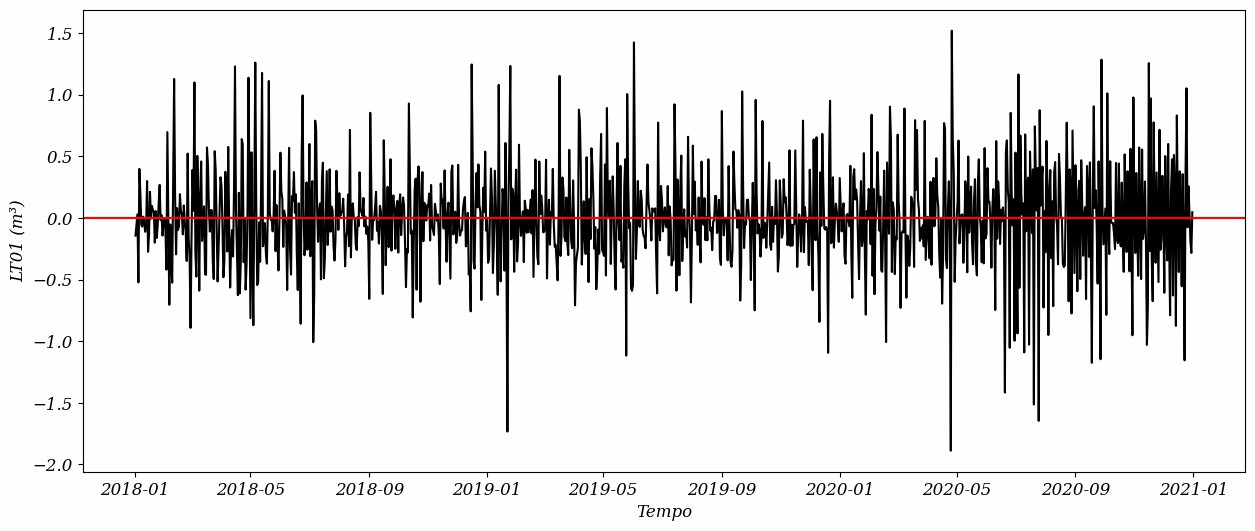
\includegraphics[width=0.9\linewidth]{Resultados/Figuras/ruido-branco}
	
	Fonte: Elaboração própria a partir de dados da SANEPAR (2018 a 2020)
\end{figure}

Da Figura \ref{fig:ruido-branco} uma série temporal pode ser ruído branco.
Uma série temporal a é ruído branco se as variáveis forem independentes e distribuídas de forma idêntica com uma média de zero.
Isto significa que todas as variáveis têm a mesma variância ($\sigma^2$) e cada valor tem correlação zero com todos os outros valores da série.
Mais adiante, é mostrado o comprimento de zeros na variável prevista. Isto conclui o \ref{etp:3}.